
% Section~\ref{sec:estep_sleep_compare} motivates the wake-sleep approach by comparing variational posteriors obtained by optimizing the ELBO against those obtained by optimizing the sleep objective. 
% Then, StarNet is tested on blended simulated stars in Section~\ref{sec:deblending_test}. 
% Finally, in Section~\ref{sec:results_on_m2}, StarNet is employed to catalog the SDSS image of the M2 globular cluster. The StarNet catalog is compared with existing cataloging methods. 

\label{sec:elbo_sleep_compare}

A simple example demonstrates that there exist shallow local optima in the ELBO~\eqref{eq:elbo} which result in unreliable catalogs. 
For this example, fitting the variational posterior using the sleep objective~\eqref{eq:sleep_obj} avoids shallow optima. 
Because the data were simulated with known PSF and background, the wake phase is not needed. 

The simulated $20\times20$ single-band image $x_{test}$ is shown in Figure~\ref{fig:toy_example}.
The image has four stars, each with the same flux. 

\begin{figure}[!h]
    \centering
    \vspace{-1em}
    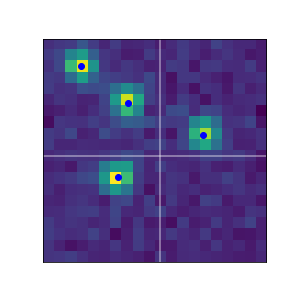
\includegraphics[width = 0.3\textwidth]{figures/vi_sleep_ex_figure.png}
    \vspace{-1.7em}
    \caption{The $20\times 20$ pixel synthetic image that we use for testing. It contains four stars and is partitioned into $10\times 10$ tiles. }
    \label{fig:toy_example}
\end{figure}

We compare three approaches. The first two approaches directly optimize the test ELBO, 
\begin{align}
\mathcal{L}_{elbo}(\eta; x_{test}) = \Expect_{q_{\eta}(z | x_{test})}\Big[\log p(x_{test}, z) - \log q_{\eta}(z | x_{test})\Big],
\label{eq:elbo_on_test}
\end{align}
while the third approach optimizes the sleep objective~\eqref{eq:sleep_obj}. 
Note that the sleep objective does not depend on $x_{test}$. 
Optimizing the sleep objective only requires sampling catalogs from the prior
and simulating images conditional on each catalog. 
The prior on the number of stars was set to be Poisson with mean $\mu = 4$. 

Figure~\ref{fig:optim_path}~(top row) charts the test ELBO~\eqref{eq:elbo_on_test} as the optimization proceeds in our three approaches.
The first approach optimizes the ELBO with stochastic gradient descent and the REINFORCE gradient estimator.
This optimization did not converge, likely due to the high variance of the REINFORCE estimator (Figure~\ref{fig:optim_path}a). 
For a lower variance gradient estimator, the second approach employed the reparameterized gradient. To employ this gradient estimator, we analytically integrated the ELBO with respect to the number of stars $N$ to remove the discrete random variable. 
See Appendix~\ref{sec:reparam_details} for details about the gradient estimators. 
Using reparameterized gradients instead of REINFORCE gradients enabled the optimization to converge to stationary points (Figure~\ref{fig:optim_path}b). 
However, for two of the six randomly initialized restarts, 
the optimization found local optima where the ELBO is lower than other restarts. 

In contrast, optimizing the sleep objective consistently converged to a similar ELBO across all restarts and appeared to avoid shallow local optima (Figure~\ref{fig:optim_path}c).
Recall that sleep phase optimization does not directly optimize the test ELBO. However, the test ELBO increases nonetheless as the variational posterior better approximates the true posterior as the optimization proceeds. 

Shallow local optima in the ELBO results in unreliable catalogs. 
The bottom row of Figure~\ref{fig:optim_path} displays the estimated locations, defined by the mode of the fitted variational distribution. 
The bottom left shows these locations after getting stuck in a shallow optimum. 
In this local optimum, the upper left tile was estimated to have two stars; however, both estimated stars were placed on the same star. 
For correct detections, one of the locations should be placed on the second star.
However, to move one estimated location to the second star, the optimization path must traverse a region where the log-likelihood is lower than the current configuration. 
The displayed configuration is a local optima where the gradient with respect to its locations is approximately zero.
In contrast, the sleep phase optimization consistently placed its mode around the four true stars. 
An example of correct detections after sleep phase optimization is shown in the bottom right of~Figure~\ref{fig:optim_path}.

\begin{figure}[!htb]
    \centering
    \begin{subfigure}[t]{0.9\textwidth}
    \centering
    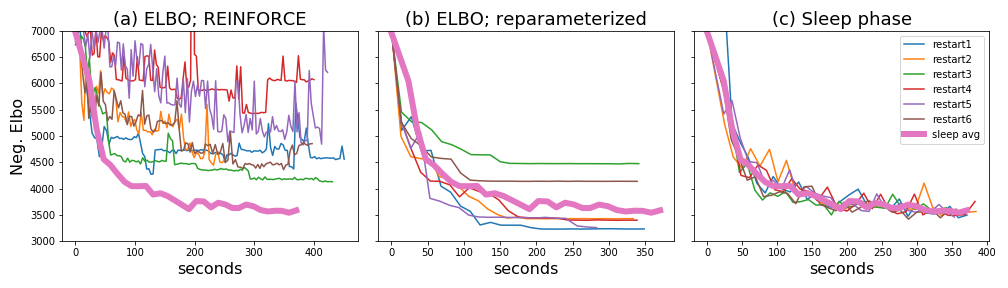
\includegraphics[width=\textwidth]{figures/optim_path_compare.png}
    \end{subfigure}
    \begin{subfigure}[t]{\textwidth}
    \centering
    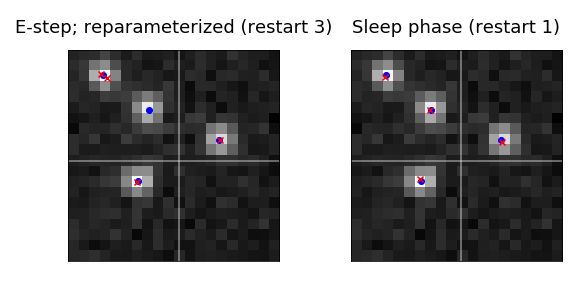
\includegraphics[width=0.55\textwidth]{figures/optim_path_detect_compare.png}
    \end{subfigure}
    \vspace{-3em}
    \caption{(Top row) The ELBO as the optimization progresses for six random restarts. 
    (Bottom row) Modal locations from two variational posteriors.
    On the left, a randomly initialized run where optimizing the ELBO with the reparameterized gradient resulted in a local optimum.
    On the right, the variational posterior 
    was optimized using the sleep phase. }
    \label{fig:optim_path}
\end{figure}

Figure~\ref{fig:gradzero_cartoon} shows a schematic of the optimization landscape as a function of locations.
Recall that locations are parameterized between 0 and 1, and the neural network returns a variational mean parameter $\mu_\ell$ for the logit-location. 
When $\mu_\ell$ is far from the correct location (in logit space), the gradient of the ELBO with respect to $\mu_\ell$ vanishes. 
To see this, observe that the PSF is nearly zero everywhere except for a few pixels around its center. Therefore, a small shift in estimated location $\mu_\ell$ does not significantly change the likelihood unless the estimated location is within a ``PSF radius" of the correct location.
On the other hand, the sleep objective is quadratic in the logit-location estimate $\mu_\ell$ (see Equation~\ref{eq:gaussian_sleep_loss}).
Thus, the further the estimated location from the correct location (in logit space), the larger the gradient. The gradient does not vanish in the sleep objective. 

\begin{figure}[!htb]
    \centering
    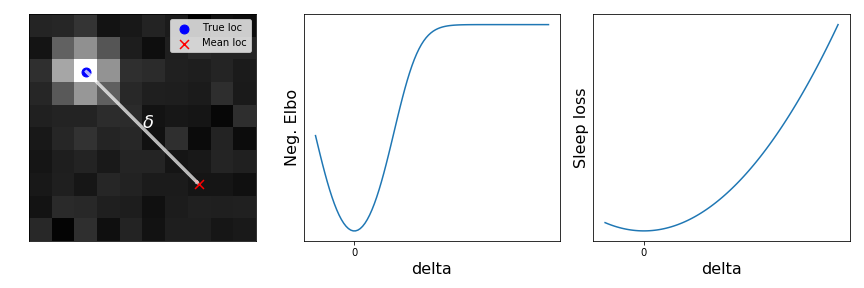
\includegraphics[width=\textwidth]{figures/gradzero_cartoon3.png}
    % \centering
    % \begin{subfigure}[t]{0.8\textwidth}
    % \centering
    % 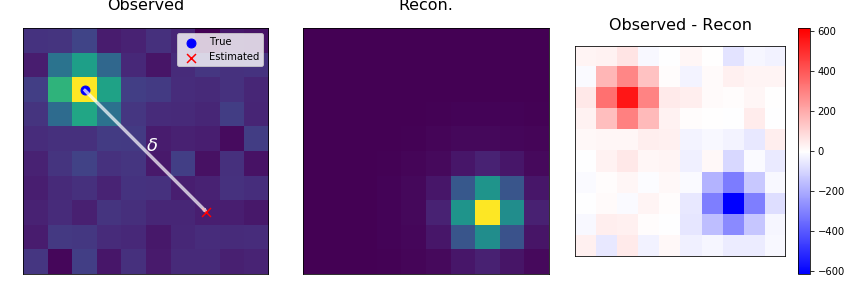
\includegraphics[width=\textwidth]{figures/gradzero_cartoon.png}
    % \end{subfigure}
    % \begin{subfigure}[t]{\textwidth}
    % \centering
    % 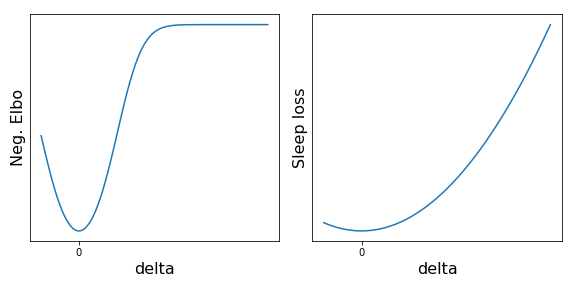
\includegraphics[width=0.55\textwidth]{figures/gradzero_cartoon2.png}
    % \end{subfigure}
    % \vspace{-3em}
    \caption{An illustration of vanishing gradients when the estimated under the variational distribution (red) is far from the correct location (blue). 
    $\delta$ denotes the difference in logit-locations. 
    For large $\delta$, the ELBO objective is flat in the estimated location, and hence gradients with respect to location is nearly zero.
    In contrast, the sleep objective is quadratic in the estimated location, and the gradient does not vanish. }
    \label{fig:gradzero_cartoon}
\end{figure}

Also, note that low-variance gradients of the ELBO for this simple example were constructed by analytically integrating out $N$. Only then could the reparameterization trick could be applied to the ELBO as the remaining latent variables are continuous. 
In this example, the variational distribution has support over only 0, 1, or 2 stars for each tile. 
Since the variational distribution factorizes over the four tiles, integrating $N$ is a summation of $3^4 = 81$ terms.
On larger images with more tiles, analytically integrating $N$ would be computationally infeasible, 
and the simple reparameterization trick would not apply. 

Figure~\ref{fig:sim_data100x100} displays our results on a larger example: a simulated $100\times 100$ image with fifty stars. 
The tiles again consisted of $10\times 10$ pixel regions. 
Optimizing the sleep objective produced nearly perfect location estimates; 
optimizing the ELBO appears to be hindered by regions with little gradient information and does not accurately produce accurate location estimates. 

\begin{figure}[!htb]
    \centering
    \begin{subfigure}[!t]{0.59\textwidth}
    \centering
    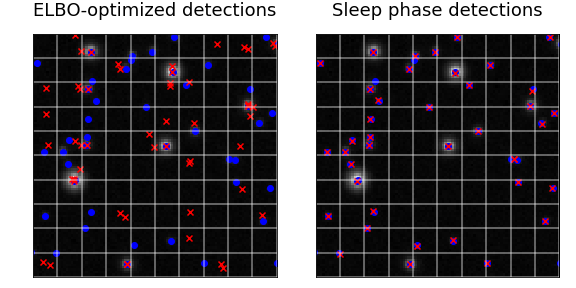
\includegraphics[width=\textwidth]{figures/optim_path_detect_compare_100x100.png}
    \end{subfigure}
    \begin{subfigure}[!t]{0.4\textwidth}
    \centering
    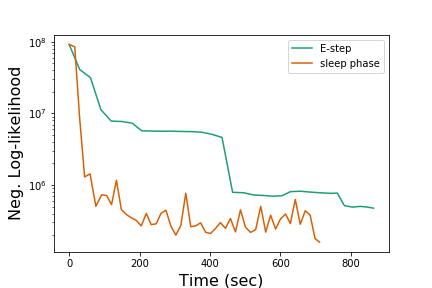
\includegraphics[width=\textwidth]{figures/optim_path_compare_100x100.png}
    \end{subfigure}
    \caption{
    (Left) Detections produced by ELBO optimization on a $100\times 100$ test image. Correct locations are blue and estimated locations are red. 
    (Middle) Detections produced by the sleep phase optimization.  
    (Right) The negative conditional log-likelihoood, $-\log p(x|\hat z)$, where $\hat z$ is the mode of the variational posterior and $x$ the 
    $100\times 100$ test image. }
    \label{fig:sim_data100x100}
\end{figure}
